% IF YOU CAN SEE THIS GO CONTRIBUTE >:(

\documentclass[letterpaper, 8pt]{extarticle}
\usepackage{amssymb,amsmath,amsthm,amsfonts}
\usepackage{multicol,multirow}
\usepackage{calc}
\usepackage{ifthen}
\usepackage[landscape]{geometry}
\usepackage[colorlinks=true,citecolor=blue,linkcolor=blue]{hyperref}

\usepackage{booktabs}
\usepackage{ulem}
\usepackage{enumitem}
\usepackage{tabulary}
\usepackage{graphicx}
\usepackage{siunitx}
\usepackage{tikz}
\usepackage{derivative}
\usepackage{svg}
\usepackage{listings}
\usepackage{setspace}
\usepackage{listings}
\usepackage{xcolor}
\usepackage{courier}
\usepackage{syntax}
\usepackage{mathpartir}
\usepackage{siunitx}
\usepackage{tabularx}

% minimal line spacing
% \setstretch{0.1}

% set borders (experimentally determined to minimize cutoff and maximize space on school printers)
\geometry{top=.25in,left=.25in,right=.25in,bottom=.35in}

% make figures work better in multicol
\newenvironment{Figure}
{\par\medskip\noindent\minipage}
{\endminipage\par\medskip}

\pagestyle{empty} % clear page

% rewrite section commands to be smaller
\makeatletter
\renewcommand{\section}{\@startsection{section}{1}{0mm}%
                                {-1explus -.5ex minus -.2ex}%
                                {0.5ex plus .2ex}%x
                                {\normalfont\small\bfseries}}
\renewcommand{\subsection}{\@startsection{subsection}{2}{0mm}%
                                {-1explus -.5ex minus -.2ex}%
                                {0.5ex plus .2ex}%
                                {\normalfont\tiny\bfseries}}
\renewcommand{\subsubsection}{\@startsection{subsubsection}{3}{0mm}%
                                {-1ex plus -.5ex minus -.2ex}%
                                {1ex plus .2ex}%
                                {\normalfont\tiny\bfseries\itshape}}
\makeatother
\setcounter{secnumdepth}{0} % disable section numbering


% disable indenting
\setlength{\parindent}{0pt}
\setlength{\parskip}{0pt plus 0.5ex}

% Custom siunitx defs
\DeclareSIUnit\noop{\relax}
\NewDocumentCommand\prefixvalue{m}{%
\qty[prefix-mode=extract-exponent,print-unity-mantissa=false]{1}{#1\noop}
}

% Shorthand definitions
\newcommand{\To}{\Rightarrow}
\newcommand{\ttt}{\texttt}
\newcommand{\ra}{\rightarrow}

% condense itemize & enumerate
\let\olditemize=\itemize \let\endolditemize=\enditemize \renewenvironment{itemize}{\olditemize \itemsep0em}{\endolditemize}
\let\oldenumerate=\enumerate \let\endoldenumerate=\endenumerate \renewenvironment{enumerate}{\oldenumerate \itemsep0em}{\endoldenumerate}
\setlist[itemize]{noitemsep, topsep=0pt, leftmargin=*}
\setlist[enumerate]{noitemsep, topsep=0pt, leftmargin=*}

\title{3GC3}

\begin{document}
\raggedright
\tiny

% make listings look nicer
\lstset{
    tabsize = 2, %% set tab space width
    showstringspaces = false, %% prevent space marking in strings, string is defined as the text that is generally printed directly to the console
    basicstyle = \tiny\ttfamily, %% set listing font and size
    breaklines = true, %% enable line breaking
    numberstyle = \tiny,
    postbreak = \mbox{\textcolor{red}{\(\hookrightarrow\)}\space}
}

\begin{center}
    {\textbf{COMPSCI 4NL3 - JOBLESS EDITION}} \\
\end{center}
% set column spacing rules
\setlength{\premulticols}{1pt}
\setlength{\postmulticols}{1pt}
\setlength{\multicolsep}{1pt}
\setlength{\columnsep}{2pt}
\begin{multicols*}{4}
    \section{Regex}

    \begin{tabularx}{\linewidth}{lX}
        \toprule
        Pattern & Matches \\
        \midrule
        $\backslash s$ & whitespace \\
        $\backslash d$ & any digit \\
        $\{N\}$ & exactly \$N\$ of the previous item \\
        $\backslash w$ & any ``word'' characters (includes numbers) \\
        $\backslash S$, $\backslash$D, $\backslash$W & anything NOT in the lowercase version of that pattern \\
        $\backslash b$ & word boundary \\
        $\string^$ & start of the string \\
        $\$$ & end of the string \\
        $A|B$ & $A$ or $B$ \\
        $[a-z]$, $[abcde]$,$[0-9]$ & any character in the brackets of specified range of characters \\
        $.$ & any character \\
        $?$ & 0 or 1 of the preceding character \\
        $*$ & 0 or more of the preceding character \\
        $+$ & 1 or more of the preceding character \\
        $.*?$ & not greedy \\
        \bottomrule
    \end{tabularx}

    \subsection{Example of Not Greedy}

    \begin{lstlisting}
    text = "<tag>I have something here</tag> <tag>but other stuff here</tag>"
    my_regex = r"<tag>.*?<\/tag>"
    re.findall(my_regex, text) = ['<tag>I have something here</tag>', '<tag>but other stuff here</tag>']
    \end{lstlisting}

    \section{Text Normalization/Pre-Processing}
    \textbf{1.} Lowercasing
    \textbf{2.} True-casing
    \textbf{3.} Punctuation Removal
    \textbf{4.} Stopword (funciton words such as articles, prepositions, conjunctions and pronouns) Removal
    \textbf{5.} Stemming (takes the stem of the word - hacky e.g. policy and police become the same word)
    \textbf{6.} Lemmatization (map all morphologically equivalent words)

    \section{Levenshtein Distance}
    \begin{tabular}{|l|l|}
        \hline
            Operation & Cost per char \\ \hline
            Insert & 1 \\ \hline
            Delete & 1 \\ \hline
            Replace & 2 \\ \hline
        \end{tabular}


    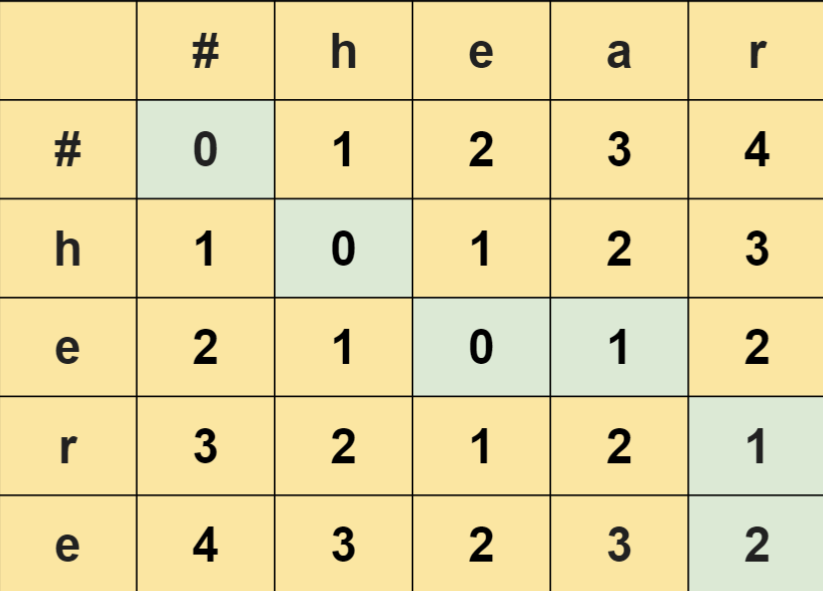
\includegraphics[width=0.5\linewidth]{LevenshteinDistance.png}

    Cell at row $i$ column $j$ represents the number of operations required from convert the first $i$ characters of our source to the first $j$ characters of our target.

    \textbf{1.} the top left cell: 0 operations to convert "" to ""
    \textbf{2.} top row/first column: increment by $1$ because it takes $n$ inserts to convert the "" to the first $n$ characters
    \textbf{3.1.} if characters in row $i$ and column $j$ are the same character, then $= \text{c}(i -1, j - 1)$
    \textbf{3.2.} otherwise $= 1 + \min( c(i, j - 1), c(i, j - 1), c(i - 1, j - 1))$


    \section{N-Gram Language Model}
    $P(w | h)  = \prod_{k = 1}^nP(w_k | w_{1 : k - 1})$
    This solution suffers from \textbf{Data Sparsity}. The exact history $h$ might not be present in the dataset we're using. Instead we can use the \textbf{Markov Assumption} and consider only the $N$ prior words in the past.

    \subsection{Unigram Model}
    $\approx P(w_n)$

    \subsection{Bigram Model}
    $ \approx P(w_n | w_{n - 1})$

    \subsection{N-gram Model}
    $ \approx P(w_n | w_{n - N + 1 : n - 1})$

    \subsection{Calculating Probabilties}
    $P(w | h) = \frac{C(hw)}{C(h^\star)} = \frac{C(hw)}{C(h)}$
    % where
    % $C(hw)$ is the count of the history followed by the word and
    % $C(h*) = C(h)$ is the count of the history followed by any word

    \textit{with Laplace (Add-One) Smoothing}
    $P^L (w | h) = \frac{C(hw) + 1}{C(h) + |V|}$

    \subsection{Text Generation}
    Chose a starting point randomly on the line of most probable n-grams.
    \textbf{Unigram model:} continue sampling words randomly
    \textbf{Bigram model:} continue sampling bigrams conditioned on previously generated word

    \subsection{Limitations}
    \textbf{- }N-grams don't do well at modeling long-term dependencies *e.g. when we get to "were", we don't know about the soup anymore*
    \textbf{- }N-grams don't do well with new sequences with similar meaning

    % \subsection{Advantages}
    % A clear paradigm to introduce
    % \textbf{- }training and test sets
    % \textbf{- }Perplexity as a metric for evaluation
    % \textbf{- }Sampling to generate sentences
    % \textbf{- }Other modifications to improve the model

    \section{Naive Bayes Text Classification}

    \textbf{- }$P(c | W) = \frac{P(W | c)P(c)}{P(W)} \approx P(W|c) P(c)$
    where $P(c)$ is the prior probability of class $c$ i.e. $\frac{\text{Count}(c)}{\text{Count}(D)}$, number of docs with class $c$ divided by count of all docs $D$

    \textbf{- }$P(W)$ we \textit{could} use a language model to get the probability of this sequence of words, but it doesn't change with respect to $c$ so it's not required to get \textbf{relative} probabilities between classes

    \textbf{- }$P(W | c)$ is a bit more complicated so we make the two following assumptions

    \subsection{Assumptions}

    \textbf{Order of the words doesn't matter: }$P(W | c) = P(w_1, \dots, w_n | c)$ such that the likelihood of the sequence given $c$ uses a Bag of Words

    \textbf{Words are conditionally independent:} $P(W | c) = P(w_1, \dots, w_n | c) = P(w_1 | c) \cdot \dots \cdot P(w_n | c)$ such that the probability of observing word $A$ does not affect the probability of observing word $B$


    \subsection{Solution Derivation}

    $\hat{c} = \arg\max_{c \in C} P(c | W)$
    $ = \arg \max _{c \in C} P(c) \prod^{N}_{i = 1}P(w_i | c)$

    it's better to operate in log space to avoid \textbf{underflow}
    $ = \arg\max_{c \in C} \log P(c) + \sum_{i = 1}^n \log P(w_i | c)$
    this is considered a \textbf{Linear Classifier}!

    To avoid division be zero, smoothing
    $P(w_i | c) = \frac{\text{count}(w_i, c) + 1}{\sum_{w \in V}( \text{count}(w, c) + 1)} = \frac{\text{count}(w _i, c) + 1}{\left(\sum_{w \in V} \text{count}(w, c)\right) + |V|}$

    \subsection{Limitation}
    It assumes conditional independence

    \section{Logistic Regression Text Classification}
    \subsection{Binary}
    Supervised learning method where $X$ is our TF-IDF counts, $Y \in \{0, 1\}$ our binary class.

    Our model is
    $P(y = 1 | x) = \sigma\left(\left(\sum_{i = 1}^n w_i x_i\right) + b\right)$
    $  = \sigma(w \cdot x + b)$
    where
    $z$ is our score i.e. $P(y = 1 | x)$,
    $w$ are our weights,
    $x$ is our features,
    $b$ is our bias,
    $\sigma$ is sigmoid function

    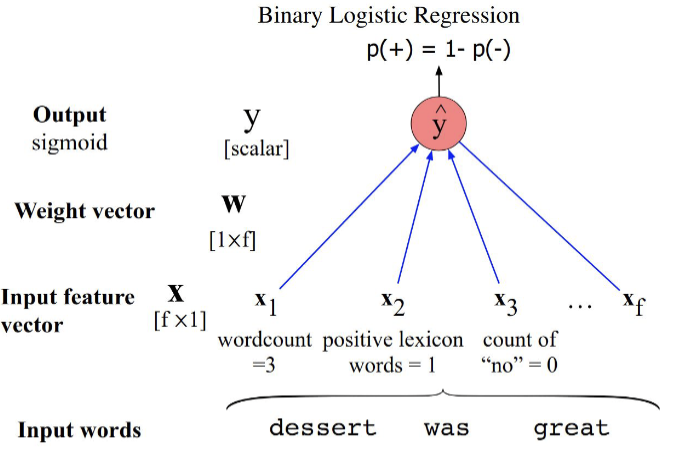
\includegraphics[width=0.8\linewidth]{BinaryLogisticRegression.png}


    \subsubsection{Example}
    \resizebox{\columnwidth}{!}{
    \begin{tabular}{p{1.2cm}|p{1.2cm}|p{1.2cm}|p{1.2cm}|p{1.2cm}|p{1.2cm}|p{1.2cm}|}
        \hline
            \textbf{Variable} & x1 & x2 & x3 & x4 & x5 & x6 \\ \hline
            \textbf{Meaning} & Count positive lexicon words & Count negative lexicon words & "No" is in document & Count 1st/2nd person pronouns & "!" is in document & $\log($word count$)$ \\ \hline
            \textbf{Value} & 3 & 2 & 1 & 3 & 0 & 4.19 \\ \hline
        \textbf{Weight} & 1.2 & -4 & 2.4 & 0.1 & 3.3 & -0.3 \\ \hline
        \end{tabular}
    }
    and \textbf{Bias} = 0.1

    Then
    $P(y^{(i)}=1| x^{(i)}) =$ %TODO
    $P(y^{(i)}=0| x^{(i)}) =$ %TODO

    \subsection{Multinomial}
    Represent $Y$ as One-Hot Encoding and use SoftMax to map values to a Probability Distribution.
    Now, we will have separate weights for each class!
    For predections, we pick the class with the highest probability.
    \subsubsection{SoftMax}
    For each element $1 \le i \le K$, $\text{softmax}(z_i) = \frac{e^{z_i}}{\sum_{j = 1}^K e^{z_j}}$
    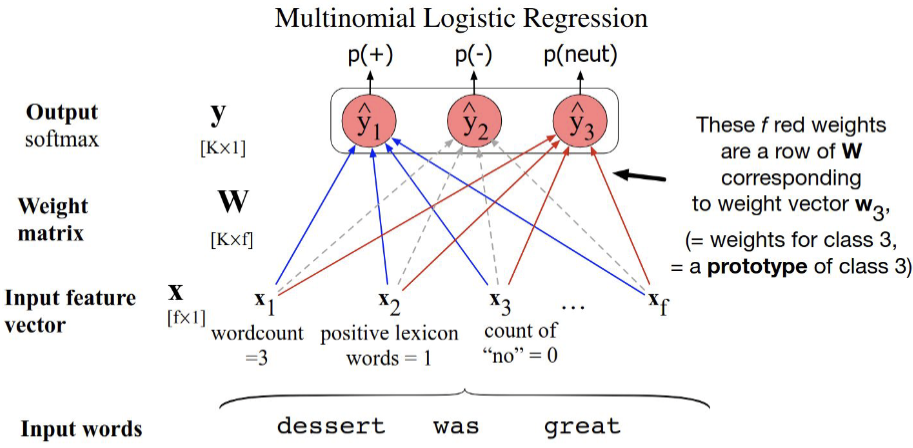
\includegraphics[width=0.8\linewidth]{MultinomialLogisticRegression.png}

    \section{Neural Network}
    Our activation functions allow us to model non-linear relationships.
    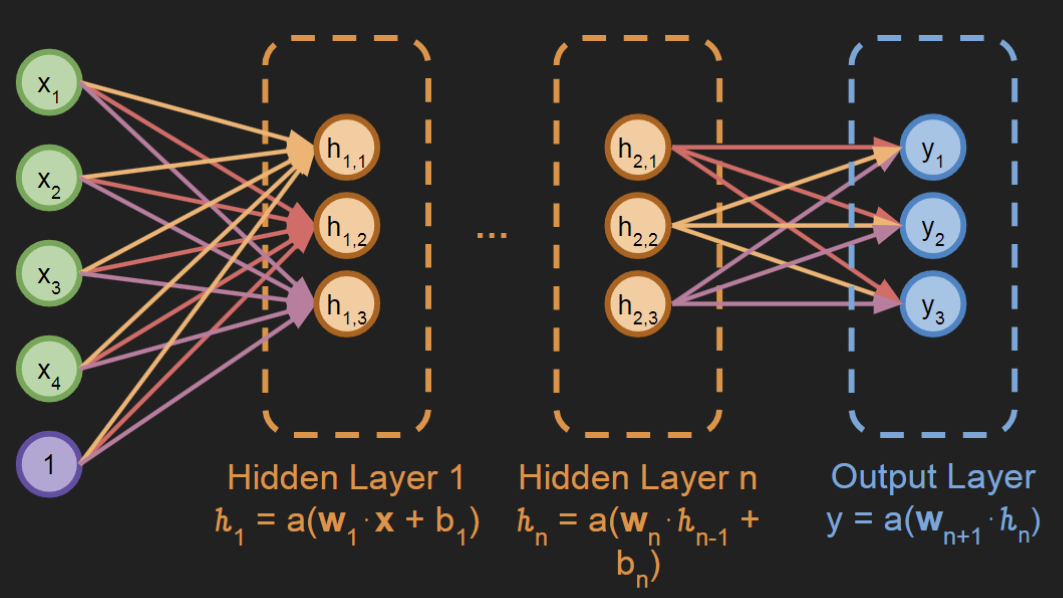
\includegraphics[width=0.5\linewidth]{NeuralNetwork.png}
    \subsection{Activation Functions}
    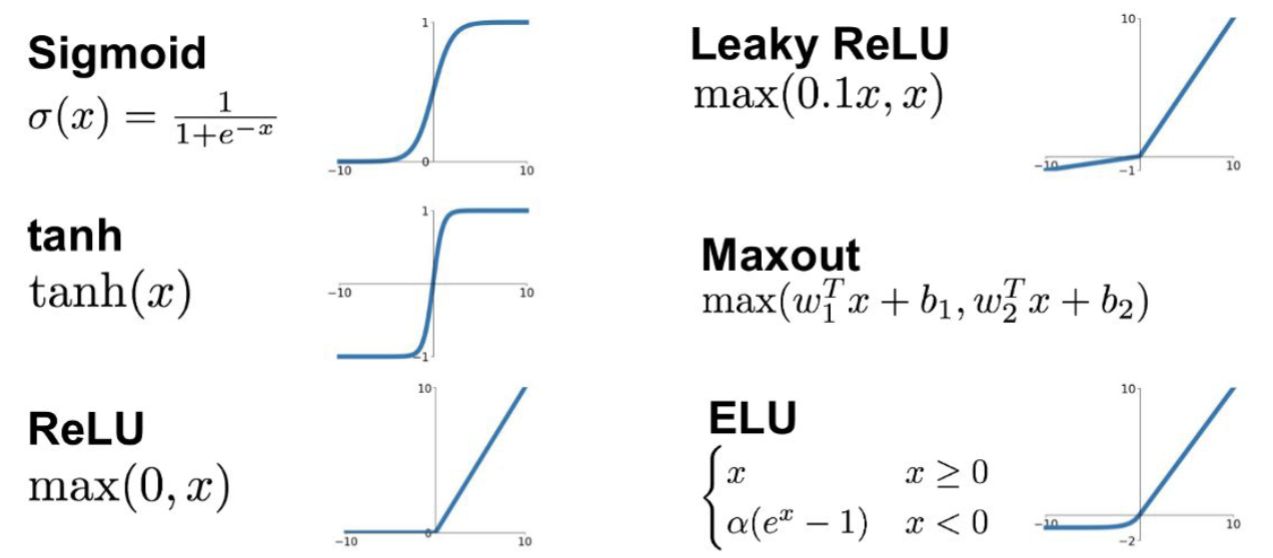
\includegraphics[width=0.5\linewidth]{ActivaitionFunctionsAndGraphs.png}
    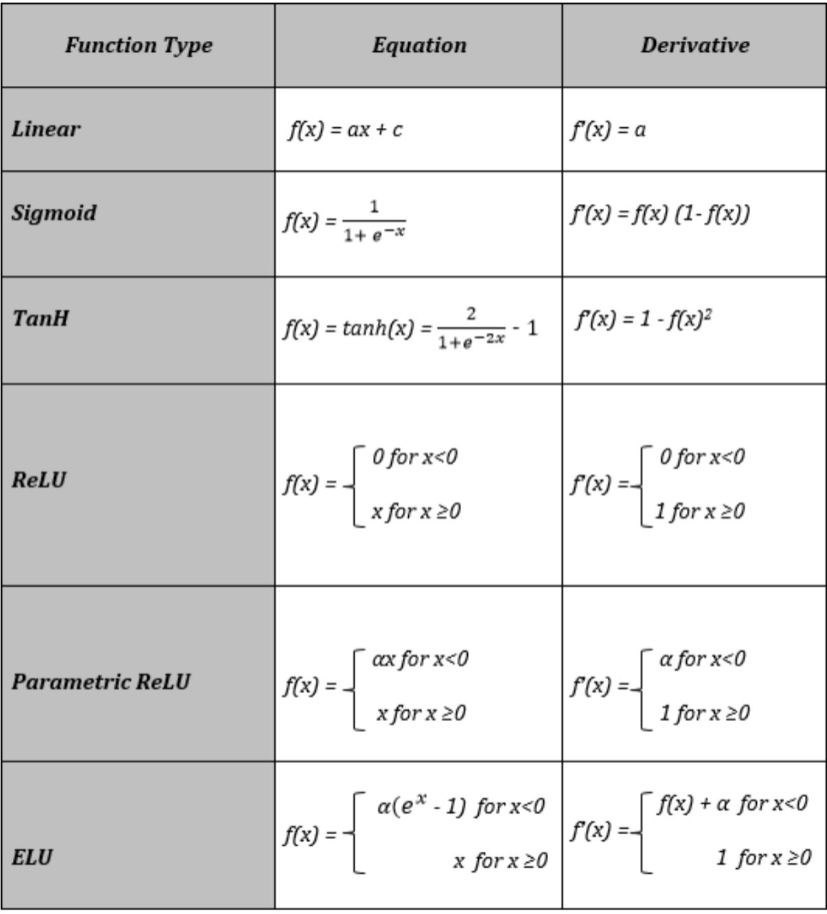
\includegraphics[width=0.5\linewidth]{ActivationFunctionsAndDerivatives.png}

    \subsection{Example}
    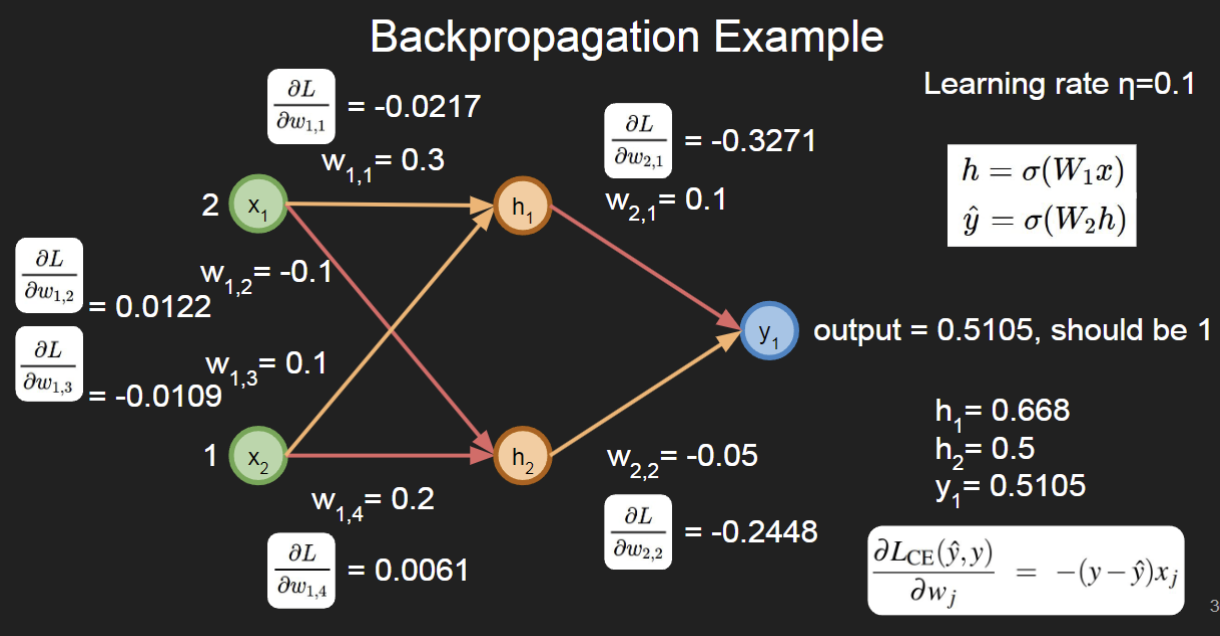
\includegraphics[width=0.5\linewidth]{BackpropagationExample.png}

    \section{Credits}
    \begin{itemize}
        \item Sarah for initial Overleaf version
    \end{itemize}
\end{multicols*}

\end{document}
